\documentclass[conference]{IEEEtran}
\IEEEoverridecommandlockouts

\usepackage{cite}
\usepackage{amsmath,amssymb}
\usepackage{graphicx}
\usepackage{booktabs}
\usepackage{algorithm}
\usepackage{algpseudocode}
\usepackage{xcolor}
\usepackage{url}
\usepackage{array}
\usepackage{tikz}
\usetikzlibrary{arrows.meta,positioning}

\newcommand{\Vsix}{V6}
\newcommand{\Vfive}{V5}

\begin{document}

\title{Source-Adjusted Candidate Feature Auditing for Group-Dependent Label Corruption: Calibration, Power, Real-Data Transfer and Mitigation}

\author{\IEEEauthorblockN{Soumya Shradha, Tanishk Gangwar, Yagya Salwan, Vivansh Garg and Chirag Joshi}
\IEEEauthorblockA{Department of Data Science and Engineering, Manipal University Jaipur, Jaipur, India}}

\maketitle

\begin{abstract}
Training labels can be corrupted in ways that depend on group membership, yet analysts are rarely told which columns are sensitive. Candidate feature auditing asks which observed feature blocks are linked to unusual label behaviour in an audit sample relative to a small trusted reference, and it must be able to abstain. We present a tested reimplementation and evaluation of a cross-fitted, source-adjusted auditor (\Vsix) that emerged from six project versions. The test multiplies out-of-fold source and label residuals, contrasts their means between candidate groups, and applies Bonferroni correction within association blocks and Benjamini--Yekutieli correction across blocks. On 10,500 synthetic datasets, \Vsix{} kept the exact 95\% upper bound of the clean alarm rate below 5\% in all 20 clean conditions and abstained on 99.0\% of random-label datasets, whereas the preceding permutation auditor (\Vfive) failed two conditions and alarmed on 23.0\% of datasets under covariate shift with a nonlinear label rule. A first power study (7,500 datasets) found at least 80\% recall at 30\% corruption but only 43--47\% at 20\%. On 2,200 record-disjoint semi-synthetic splits of COMPAS and German Credit, \Vsix{} recovered injected race-linked corruption in 59.5\% of COMPAS splits, where \Vfive{} could not test race at all. After a \Vsix{} flag, audit-guided reweighting reduced the corrupted group's prediction bias from 14.3 to 1.6 percentage points. In a pre-registered study of 5,000 further real-data splits, \Vsix{} also kept the upper bound below 5\% under clean and age-shifted sampling. Sensitivity to mild corruption remains limited.
\end{abstract}

\begin{IEEEkeywords}
algorithmic auditing, label bias, cross-fitting, conditional independence testing, false discovery rate, fairness
\end{IEEEkeywords}

\section{Introduction}
Labels are often produced by processes that treat groups differently. Re-arrest records used as recidivism labels depend on where policing is concentrated~\cite{angwin2016machine,chouldechova2017fair}, and recorded credit outcomes reflect earlier lending decisions. A model trained on such labels reproduces the pattern even when the protected attribute is removed~\cite{mehrabi2021survey}. Most corrective methods assume that the affected group is specified in advance~\cite{kamiran2012data,feldman2015certifying,jiang2020identifying,blum2020recovering}. An analyst may instead receive a table with many columns and no statement of which ones are sensitive.

\emph{Candidate feature auditing} addresses a narrower, earlier question. Given an \emph{audit} sample whose labels are under review and a smaller \emph{trusted} sample with reliable labels, which observed feature blocks, if any, are linked to a label difference between the two sources that the other features do not explain? Three tasks must be kept apart. \emph{Ranking} orders features by a score. \emph{Detection} decides, with error control, whether any feature warrants review, and may abstain. \emph{Mitigation} changes the data and must be evaluated on its own. Ranking alone is insufficient, since pure noise also has a top-ranked feature.

Our project developed this auditor over six versions~\cite{salwan2026report,team2026manuscript} (Table~\ref{tab:history}). The first version ranked features without a calibrated null; the second added one but was later found to leak information. Versions 3--5 compared audit labels with an independent trusted calibration sample using conditional source permutations. They controlled alarms in matched populations but alarmed under clean covariate shift. \Vsix{} replaced the permutation null with a cross-fitted residual test that models source membership. Its archived study passed 24 of 25 calibration conditions; because the protocol required every condition to pass, corruption power was never measured.

This paper makes four contributions. (i)~A tested reimplementation of the \Vsix{} auditor and the \Vfive{} comparator from the written method, with a per-group effect size based on partialling out~\cite{robinson1988root,chernozhukov2018double}. (ii)~A paired calibration study on 10,500 datasets in 21 conditions, including covariate shift combined with a nonlinear label rule. (iii)~The first power study of \Vsix{} (7,500 datasets), showing where the 80\% recall target is and is not met. (iv)~Semi-synthetic real-data transfer on COMPAS and German Credit with record-disjoint splits, a pre-registered real-data calibration study, and an evaluation of audit-guided mitigation on clean held-out labels. Section~\ref{sec:discussion} states what the evidence does not establish.

\begin{table}[t]
\caption{Development history of the auditor~\cite{salwan2026report}}
\label{tab:history}
\centering
\footnotesize
\setlength{\tabcolsep}{3pt}
\begin{tabular}{@{}l>{\raggedright\arraybackslash}p{3.3cm}>{\raggedright\arraybackslash}p{3.8cm}@{}}
\toprule
Ver. & Main change & Finding in the archived study\\
\midrule
V1 & local neighbour disparity, top-3 ranking & selected three features in every null control\\
V2 & empirical null, BH, gated reweighting & leakage and adaptive draws; claims withdrawn\\
V3 & trusted calibration sample, blocks, coherent score & 9/9 matched clean cells passed; no 20\% cell reached 80\% recall\\
V4 & trusted-sample allocation, BY vs.\ Holm & recall up in 18/18 cells; primary failed calibration\\
V5 & frozen validation, 21 conditions & 18 matched passed; mean-shift controls failed\\
V6 & cross-fitted residual test & 24/25 passed (upper bound 5.39\%); power not run\\
\bottomrule
\end{tabular}
\end{table}

\section{Related Work}
\emph{Label noise.} Classical work models noise as instance- or class-conditional and aims at robust learning or data cleaning~\cite{frenay2014classification,northcutt2021confident}. Our target is different: a group-linked difference between two sources, reported as a review signal rather than corrected automatically.

\emph{Label bias and fairness.} Jiang and Nachum reweight examples to correct biased labels~\cite{jiang2020identifying}, and Blum and Stangl analyse when fairness constraints recover from biased labels~\cite{blum2020recovering}. Both assume that the group is known. Reweighing and disparate-impact repair also require the protected attribute~\cite{kamiran2012data,feldman2015certifying}. Methods for fairness without demographics, such as distributionally robust optimisation~\cite{hashimoto2018fairness} and adversarially reweighted learning~\cite{lahoti2020fairness}, change the training objective. They do not decide, with error control, whether a specific feature is implicated. We use group criteria such as equalised odds~\cite{hardt2016equality} only to evaluate downstream models; the project's first version drew on individual fairness~\cite{dwork2012fairness}.

\emph{Testing.} The \Vsix{} statistic is closely related to the generalised covariance measure of Shah and Peters~\cite{shah2020hardness}, which tests conditional independence through the mean of products of regression residuals. It also follows the cross-fitting and partialling-out ideas of double machine learning~\cite{chernozhukov2018double,robinson1988root}. Instead of a single global test of $S \perp Y \mid X$, \Vsix{} contrasts residual-product means between groups of a candidate feature, so a source difference shared by all groups does not produce a flag on its own. Multiplicity across blocks is handled by the Benjamini--Yekutieli (BY) procedure~\cite{benjamini2001control}, which is valid under arbitrary dependence. Holm~\cite{holm1979simple} and Benjamini--Hochberg~\cite{benjamini1995controlling} appear in earlier versions. Covariate shift without a change in $P(Y\mid X)$~\cite{shimodaira2000improving} is exactly the setting in which naive source comparisons raise false alarms.

\section{Problem Setting}
Let $X$ denote the observed features, $Y\in\{0,1\}$ the observed label and $S\in\{0,1\}$ the source, with $S=0$ for trusted records (clean labels) and $S=1$ for audit records. Each candidate feature $j$ induces groups (quantile bins or category levels) that are fixed before any outcome is examined. The auditor is never told which columns are sensitive.

\emph{Clean null.} The audit labels are uncorrupted if $P(Y{=}1\mid X,S{=}1)=P(Y{=}1\mid X,S{=}0)$. The covariate distribution may still differ between the sources (population shift). \emph{Group-dependent corruption.} In the audit source, a fraction $c$ of eligible labels inside a group $g^\ast$ are flipped, so the conditional label distribution differs between sources only within $g^\ast$.

\emph{Output.} The auditor returns flagged feature blocks with effect sizes and adjusted $p$-values, or the abstention ``No statistically supported candidate detected.'' A flag is a prompt for human review, not proof of discrimination, and an abstention does not certify the data.

\emph{Gates.} The project protocol~\cite{salwan2026report} defines three gates. (G1)~In every clean condition, the exact two-sided 95\% Clopper--Pearson~\cite{clopper1934use} upper bound on the alarm rate (the probability of any flag) must lie below 5\%. (G2)~Under random labels, the lower bound on the abstention rate must be at least 90\%. (G3)~Recall of the corrupted block must reach at least 80\% in each 20--30\% corruption cell, and is interpreted only after G1 and G2 pass.

\section{Method}
\begin{figure}[t]
\centering
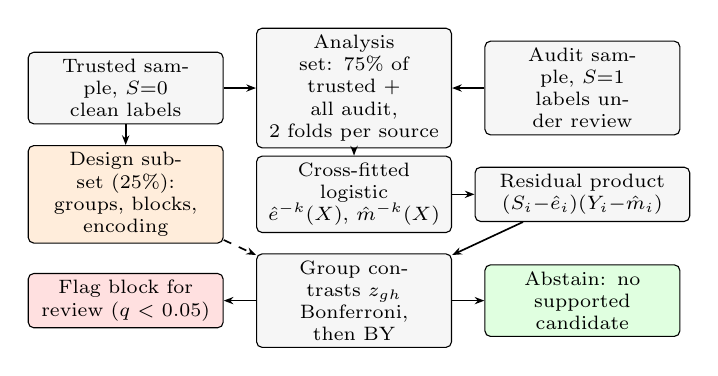
\begin{tikzpicture}[font=\scriptsize,
  box/.style={draw, rounded corners=2pt, align=center, inner sep=2.5pt, text width=2.3cm, fill=gray!7},
  arr/.style={-{Stealth[length=3.5pt]}, semithick}]
\node[box] (T) at (0,0) {Trusted sample, $S{=}0$\\clean labels};
\node[box] (X) at (2.9,0) {Analysis set: 75\% of\\trusted + all audit,\\2 folds per source};
\node[box] (A) at (5.8,0) {Audit sample, $S{=}1$\\labels under review};
\node[box, fill=orange!14] (D) at (0,-1.35) {Design subset (25\%):\\groups, blocks,\\encoding};
\node[box] (M) at (2.9,-1.35) {Cross-fitted logistic\\$\hat e^{-k}(X)$, $\hat m^{-k}(X)$};
\node[box, text width=2.55cm] (R) at (5.8,-1.35) {Residual product\\$(S_i{-}\hat e_i)(Y_i{-}\hat m_i)$};
\node[box] (C) at (2.9,-2.7) {Group contrasts $z_{gh}$\\Bonferroni, then BY};
\node[box, fill=red!12] (F) at (0,-2.7) {Flag block for\\review ($q<0.05$)};
\node[box, fill=green!12] (N) at (5.8,-2.7) {Abstain: no\\supported candidate};
\draw[arr] (T) -- (X); \draw[arr] (A) -- (X); \draw[arr] (T) -- (D);
\draw[arr] (X) -- (M); \draw[arr] (M) -- (R); \draw[arr] (R) -- (C);
\draw[arr, dashed] (D) -- (C);
\draw[arr] (C) -- (F); \draw[arr] (C) -- (N);
\end{tikzpicture}
\caption{The \Vsix{} audit. The design subset fixes groups and blocks (dashed) before any analysis label is used; every analysis record is predicted by models that did not train on it.}
\label{fig:pipeline}
\end{figure}

\subsection{Design geometry}
A random 25\% of the trusted records forms a \emph{design subset}. Its labels are used only to fix three things: candidate groups, feature blocks and preprocessing. Numeric features with more than six distinct values are cut into quartile bins. Other features use each level that holds at least 3\% of design records, with the remaining levels merged. Preprocessing uses median imputation, standardisation and one-hot encoding. Association is $|\rho_{\text{Spearman}}|$ for numeric pairs and Cram\'er's $V$ between group codes otherwise. Blocks are the connected components of the graph with an edge wherever association is at least $0.60$. The archived study set this threshold after showing that a binary proxy flipped for 10\% of records at 25\% prevalence has population association $\approx0.756$, which an earlier 0.80 threshold missed~\cite{salwan2026report}. Our implementation reproduces that value.

\subsection{Cross-fitted residual contrasts}
The remaining trusted records and all audit records form the analysis set, which is split into two folds within each source. For fold $k$, $\ell_2$-regularised logistic regressions fitted on the other fold give $\hat m^{-k}(x)\approx P(Y{=}1\mid x)$ and $\hat e^{-k}(x)\approx P(S{=}1\mid x)$ from all features. For record $i$ in fold $k(i)$,
\begin{equation}
r_i=\bigl(S_i-\hat e^{-k(i)}(X_i)\bigr)\bigl(Y_i-\hat m^{-k(i)}(X_i)\bigr).
\label{eq:r}
\end{equation}
Under the clean null with correct nuisance functions, $E[r\mid X]=0$, so the mean of $r$ is zero within every group~\cite{shah2020hardness}. For groups $g$ and $h$ of feature $j$,
\begin{equation}
z_{gh}=\frac{\bar r_g-\bar r_h}{\sqrt{s_g^2/n_g+s_h^2/n_h}},
\label{eq:z}
\end{equation}
with a two-sided normal $p$-value. A group is \emph{supported} if it has at least 20 analysis records from each source, including at least 10 per source in each fold; each source also needs at least 100 analysis records. Unsupported contrasts keep $p=1$ and remain in the family. The $p$-value of block $b$ is $\min(1, M_b\min p)$ over its $M_b$ contrasts (Bonferroni). BY is then applied across blocks, and supported blocks with $q<0.05$ are flagged (Fig.~\ref{fig:pipeline}, Algorithm~\ref{alg:v6}).

\subsection{Per-group effect size}
For reporting, we use the partialling-out estimate~\cite{robinson1988root}
\begin{equation}
\hat\theta_g=\frac{\sum_{i\in g} r_i}{\sum_{i\in g}\bigl(S_i-\hat e_i\bigr)^2},
\label{eq:theta}
\end{equation}
the coefficient from regressing the label residual on the source residual within group $g$. It estimates the audit-minus-trusted difference in label probability inside $g$ after both nuisance models have used $X$; we report it with a plug-in normal interval that treats the denominator as fixed. A source effect common to all groups, such as a different base rate, is not group-specific and cancels in~(\ref{eq:z}).

\begin{algorithm}[t]
\caption{\Vsix{} candidate feature audit}
\label{alg:v6}
\footnotesize
\begin{algorithmic}[1]
\State Draw design subset $D$ (25\% of trusted); fit groups, blocks (assoc.\ $\ge 0.60$) and encoding on $D$ only
\State Analysis set $A \gets$ (trusted $\setminus D$) $\cup$ audit; split each source into folds 1, 2
\For{$k \in \{1,2\}$}
  \State Fit $\hat m^{-k}$, $\hat e^{-k}$ (logistic) on fold $3-k$; predict fold $k$
\EndFor
\State $r_i \gets (S_i-\hat e_i)(Y_i-\hat m_i)$ for all $i \in A$
\For{each feature $j$ and group pair $(g,h)$}
  \State $p_{gh} \gets$ normal test of (\ref{eq:z}) if both groups supported, else $1$
\EndFor
\State $p_b \gets \min(1, M_b \min_{(g,h)\in b} p_{gh})$; \ $q \gets \mathrm{BY}(p_b)$
\State \Return blocks with $q_b<0.05$, or ``No statistically supported candidate detected''
\end{algorithmic}
\end{algorithm}

\subsection{Comparator (V5)}
\Vfive{}~\cite{salwan2026report} fits, on design data, a risk model that excludes the block and forms four risk strata. Within each stratum $s$ and group $g$ it computes $d(s,g)$, the audit-minus-calibration positive rate, and the coherent score $T=\max_g\sum_s w(s)d(s,g)-\min_g\sum_s w(s)d(s,g)$ with harmonic-support weights. The block maximum is calibrated with $B=1{,}999$ hypergeometric source permutations within (block pattern $\times$ stratum) cells. A stratum is eligible only if \emph{every} group has at least 10 records from each source.

\subsection{Audit-guided mitigation}
Mitigation runs only after a flag. For the lead feature of the flagged block, a logistic model trained on trusted records predicts clean probabilities. Within each group $g$ of the audit records, let $E_g$ be the mean predicted probability and $O_g$ the observed positive rate. Positives receive weight $E_g/O_g$ and negatives $(1-E_g)/(1-O_g)$. Weights are clipped to $[0.5,2]$ and normalised, and the intervention is rejected if Kish's effective sample size~\cite{kish1965survey} falls below 70\% of $n$.

\section{Experimental Design}
\subsection{Synthetic family}
Five legitimate predictors $x_1,\dots,x_5\sim N(0,1)$ enter the logit with coefficients $(0.8,-0.6,0.5,0.4,-0.3)$ and intercept $-0.3$. A binary group $a$ has prevalence 25\% and a legitimate effect of 0.3; a proxy $p$ equals $a$ flipped with probability 10\%; and five $N(0,1)$ columns carry no signal. By default there are 5,000 audit and 1,667 trusted records. Corruption relabels audit records with $a=1$ and clean label 1 as 0 with probability $c$. A shift adds $\delta$ to the audit mean of $x_1$. The nonlinear rule adds $0.6(x_1^2-1)+0.5x_2x_3$ to the logit.

The calibration study covers 20 clean conditions. They vary proxy noise (0, 30, 50\%), audit size (1,000; 10,000), trusted size (833; 3,333), prevalence (10, 50\%), 20 noise columns, nonlinear labels, 30\% missingness and correlated nuisance columns ($\rho=0.7$). They also include shifts $\delta\in\{0.75,1.50\}$ and four combinations of $\delta=1.50$ with nonlinear labels, correlated nuisance columns, 20 noise columns or 10\% prevalence. A random-label control completes the set, with 500 datasets per condition (10,500 in total). The power study crosses $c\in\{10,20,30,40\}\%$ with proxy noise $\{0,10,30\}\%$ and adds three cells: $c=30\%$ with $\delta=1.5$, and $c\in\{20,30\}\%$ with 10,000 audit records (7,500 datasets). Both methods run on every dataset, and paired differences are tested with exact McNemar tests~\cite{mcnemar1947note}.

\subsection{Real-data transfer}
We use COMPAS (6,172 defendants after ProPublica's filtering~\cite{angwin2016machine}; label two-year re-arrest; nine features) and German Credit (1,000 applicants~\cite{hofmann1994statlog}; 20 features; label bad risk). Each split first draws a 25\% clean test set. Of the remainder, 30\% becomes trusted, and 70\% of what is left is sampled as audit, either uniformly or with probability $\propto\exp(\gamma z_{\text{age}})$ for a clean shift with $\gamma\in\{1.0,1.5\}$. Corruption relabels audit negatives as positives with probability $c$ in the target group: race = African-American in COMPAS, and female (divorced, separated or married) in German Credit. We draw 200 splits per condition (2,200 in total). Because 200 splits cannot resolve alarm rates near 5\%, a second study repeats the five clean and age-shift conditions with 1,000 fresh splits each (5,000 in total). Its protocol, seeds and gate were committed to version control before the first run.

\subsection{Mitigation evaluation and protocol}
In corrupted splits where \Vsix{} flagged, we compare five strategies: training on the audit labels (baseline), audit-guided reweighting, dropping the flagged block, training on trusted records only, and an oracle trained on the clean audit labels. Each is fitted with logistic regression (LR) and a 100-tree random forest (RF)~\cite{pedregosa2011scikit}. On clean test labels we report AUC, the equalised-odds (EO) gap, $\max(|\Delta\mathrm{TPR}|,|\Delta\mathrm{FPR}|)$ between the target group and the rest~\cite{hardt2016equality}, and the group prediction bias, defined as the mean predicted probability minus the clean positive rate in the target group.

The code, gates and condition list were fixed before the main runs. A 100-repetition pilot on four conditions preceded them, after which two trusted-size conditions were added; no auditor code was changed. This is therefore a development and validation study by the method's developers, not a locked confirmation study; only the second real-data calibration study was formally pre-registered.

\subsection{Implementation and interactive tool}
The auditor is a Python package built on NumPy, pandas, SciPy and scikit-learn~\cite{pedregosa2011scikit}. Its 31 automated tests include reproductions of the interval values quoted in the project protocol, such as the 5.39\% upper bound for 17 alarms in 500 runs and the 0.756 proxy association. A web application exposes the same code in four views. A \emph{synthetic lab} runs clean, corrupted and shifted scenarios with \Vsix{} and \Vfive{} side by side and reveals the ground truth afterwards. A \emph{real-data audit} accepts COMPAS, German Credit or an uploaded CSV, injects corruption or shift, and then trains the downstream models. A \emph{calibration} view runs live Monte-Carlo alarm studies with exact bounds, and a \emph{method} view states the limits of a flag. Every audit exports a JSON report with all contrasts, supports and adjusted $p$-values. The implementation, study scripts and per-run records are available from the authors.

\section{Results}
\subsection{Calibration}
Fig.~\ref{fig:cal} and Table~\ref{tab:gates} summarise the study. \Vsix{} passed G1 in all 20 clean conditions, with alarm rates of 0.6--3.0\%. Its largest upper bound, 4.90\%, came with only 833 trusted records (15/500 alarms). It abstained on 495 of 500 random-label datasets (lower bound 97.7\%), passing G2. \Vfive{} passed 18 of 20 conditions. It failed with 833 trusted records (upper bound 5.14\%) and under shift with nonlinear labels, where it alarmed on 115 of 500 datasets (23.0\%, CI 19.4--26.9\%) against 12 of 500 for \Vsix{}. On the same datasets, 110 runs alarmed under \Vfive{} alone and 7 under \Vsix{} alone (exact McNemar $p<10^{-24}$). In our generator, \Vfive{} passed both linear shift conditions.

\Vfive{} raised no alarms with 20 noise columns, but this is not evidence of good calibration. With $B=1{,}999$, the smallest attainable $p$ is $1/2000$, which exceeds the BY rank-one cutoff for 26 blocks, $0.05/(26\sum_{i\le 26}i^{-1})\approx0.000499$. \Vfive{} therefore cannot flag an isolated block in that setting~\cite{salwan2026report}. The median run time per dataset was 0.19\,s for \Vsix{} and 0.38\,s for \Vfive{} (Intel Core i5-12450H, ten studies in parallel).

\begin{figure}[t]
\centering
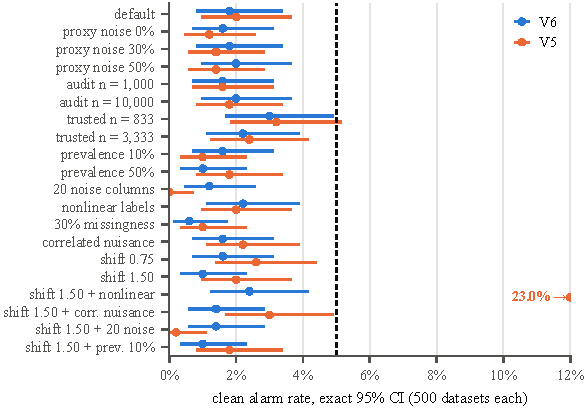
\includegraphics[width=\columnwidth]{figures/fig_calibration.pdf}
\caption{Clean alarm rate per condition (paired, 500 datasets each) with exact 95\% intervals. The dashed line marks the 5\% gate on the upper bound; the arrow gives the \Vfive{} rate beyond the axis.}
\label{fig:cal}
\end{figure}

\begin{table}[t]
\caption{Results against the protocol gates}
\label{tab:gates}
\centering
\footnotesize
\setlength{\tabcolsep}{4pt}
\begin{tabular}{@{}lcc@{}}
\toprule
Endpoint & \Vsix & \Vfive\\
\midrule
G1: clean conditions passed (synthetic) & 20/20 & 18/20\\
\quad largest upper bound & 4.90\% & 26.9\%\\
G2: random-label abstention & 99.0\% & 99.2\%\\
\quad lower bound & 97.7\% & 98.0\%\\
G3: cells $\ge$80\% recall, $c\in\{20,30\}\%$, $n{=}5$k & 3/6 & 3/6\\
\quad recall at $c=20\%$, $n=10$k & 83.8\% & 81.2\%\\
G1 on real data (pre-registered, 5 cond.) & 5/5 & 5/5\\
\quad COMPAS clean alarms (1,000 splits) & 2.1\% & 0.9\%\\
COMPAS recall of race, $c=30\%$ & 59.5\% & 0.5\%\\
\bottomrule
\end{tabular}
\end{table}

\subsection{Power}
At $n=5{,}000$ (Fig.~\ref{fig:power}), \Vsix{} recall was 3.0--5.4\% at 10\% corruption, 42.6--46.8\% at 20\%, 88.0--91.6\% at 30\% and at least 99.6\% at 40\%. G3 is therefore met at 30\% but not at 20\%; with 10,000 audit records, recall at 20\% rose to 83.8\%. The paired comparisons were mixed. \Vsix{} was better with a noisy proxy (at $c=20\%$ and 30\% noise, 59 vs.\ 7 discordant runs, $p<10^{-10}$). \Vfive{} was better at $c=20\%$ with an exact proxy (39 vs.\ 17, $p=0.005$) and under shift (93.4\% vs.\ 81.6\%; 62 vs.\ 3, $p<10^{-14}$). Off-target selections stayed at or below 5.8\%, except at 30\% proxy noise. There the proxy's association with $a$ is about 0.35, below the 0.60 threshold, so $p$ forms its own block. Selecting it is a genuine proxy signal, but we count it as off-target (up to 24.6\% at $c=40\%$).

\begin{figure}[t]
\centering
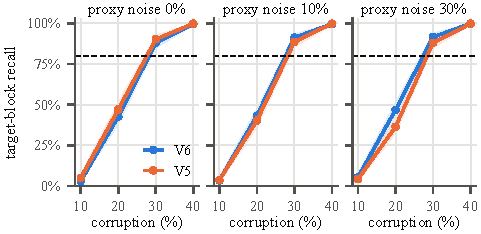
\includegraphics[width=\columnwidth]{figures/fig_power.pdf}
\caption{Recall of the corrupted block at $n=5{,}000$ (500 datasets per point, shaded 95\% intervals). The dashed line marks the 80\% target.}
\label{fig:power}
\end{figure}

\subsection{Effect-size accuracy}
For the corrupted group $a=1$, the realised gap is the mean of $Y-Y^\ast$ over audit records with $a=1$. Over 300 datasets per corruption level (Table~\ref{tab:theta}), $\hat\theta_g$ from~(\ref{eq:theta}) was essentially unbiased, and its 95\% interval covered the realised gap in 95.0--97.0\% of datasets. The flag can therefore be read with a calibrated magnitude: at $c=30\%$, ``audit labels in $a{=}1$ are about 15 percentage points lower than trusted labels after adjustment.''

\begin{table}[t]
\caption{Recovery of the injected gap by $\hat\theta_g$ for $a=1$ (300 datasets per row)}
\label{tab:theta}
\centering
\footnotesize
\setlength{\tabcolsep}{5pt}
\begin{tabular}{@{}ccccc@{}}
\toprule
$c$ & realised gap & mean $\hat\theta_g$ & SD of $\hat\theta_g$ & 95\% CI coverage\\
\midrule
0\% & 0.000 & 0.001 & 0.027 & 95.3\%\\
20\% & $-0.100$ & $-0.100$ & 0.028 & 95.0\%\\
30\% & $-0.150$ & $-0.147$ & 0.028 & 95.3\%\\
40\% & $-0.201$ & $-0.198$ & 0.026 & 97.0\%\\
\bottomrule
\end{tabular}
\end{table}

\subsection{Real-data transfer}
On COMPAS (Fig.~\ref{fig:real}), \Vsix{} recovered race in 0.5\%, 16.0\% and 59.5\% of splits at $c=10$, 20 and 30\%, and in 59.5\% at 30\% combined with the age shift. \Vfive{} recall never exceeded 0.5\%. In every split we inspected, \Vfive{} marked race as unsupported. The merged Asian and Native-American group (42 defendants) never reaches 10 records per source per stratum, so \Vfive's all-groups rule removes the whole feature from testing. \Vsix's pairwise support still compares the supported groups. On the smaller German Credit dataset, \Vsix{} recall was 4.0\% at $c=30\%$ and 35.5\% at $c=50\%$; \Vfive{} recall was zero.

In the first study, \Vsix{} alarmed on 5 of 200 clean COMPAS splits (upper bound 5.74\%), too few splits to settle G1. In the pre-registered study, \Vsix{} passed G1 in all five conditions. On COMPAS it alarmed on 2.1\%, 1.8\% and 1.7\% of 1,000 clean, $\gamma=1.0$ and $\gamma=1.5$ splits (largest upper bound 3.19\%); on German Credit, 0.6\% and 0.4\% (upper bounds at most 1.30\%). \Vfive{} also passed, with fewer alarms on clean COMPAS (0.9\%; 16 vs.\ 4 discordant splits, $p=0.012$). Part of that difference is that \Vfive{} cannot test race. \Vsix's false alarms were spread across features. The three juvenile-count features, whose non-zero groups are small and skewed, accounted for 24 of the 58 flagged blocks.

\begin{figure}[t]
\centering
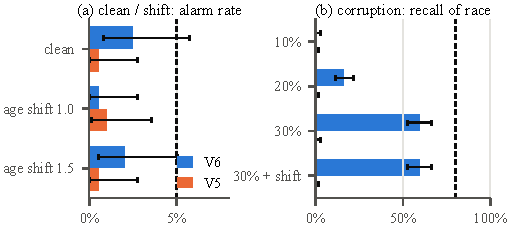
\includegraphics[width=\columnwidth]{figures/fig_realdata.pdf}
\caption{COMPAS semi-synthetic transfer with record-disjoint splits and exact 95\% intervals: (a) alarm rate without corruption, with and without an age shift (pre-registered study, 1,000 splits per bar); (b) recall of race at corruption rate $c$ (200 splits per bar).}
\label{fig:real}
\end{figure}

\subsection{Mitigation}
Table~\ref{tab:mit} reports the 122 COMPAS splits at $c=30\%$ where \Vsix{} flagged. Reweighting reduced the group prediction bias from 0.143 to 0.016 with LR and from 0.114 to 0.016 with RF (oracle: 0.002 and $-0.007$). AUC rose by 0.016 and 0.008, and the EO gap fell from 0.652 to 0.387 (LR) and from 0.474 to 0.284 (RF). The project's criteria (lower EO gap, AUC loss $\le0.02$, ESS $\ge70\%$) were met in 97.5\% (LR) and 98.4\% (RF) of these splits. Dropping the flagged block gave the smallest EO gap but left a bias of 0.067. Removing race changes predictions in ways unrelated to the injected corruption (the clean-label oracle keeps race as an input and has a larger EO gap), so the EO gap alone can reward an intervention that leaves the corruption in place. Training on trusted records only was competitive (bias $\approx0$, LR EO gap 0.295), because the trusted sample (about 1,389 records) is large for this task. On German Credit at $c=50\%$ (72 flagged splits), reweighting reduced the LR bias from 0.323 to 0.091 and raised AUC by 0.029.

\begin{table}[t]
\caption{Mitigation on COMPAS, $c=30\%$, 122 flagged splits (clean test labels; means)}
\label{tab:mit}
\centering
\footnotesize
\setlength{\tabcolsep}{2.6pt}
\begin{tabular}{@{}lcccccc@{}}
\toprule
& \multicolumn{2}{c}{AUC} & \multicolumn{2}{c}{EO gap} & \multicolumn{2}{c}{Group bias}\\
\cmidrule(lr){2-3}\cmidrule(lr){4-5}\cmidrule(l){6-7}
Strategy & LR & RF & LR & RF & LR & RF\\
\midrule
Baseline (audit labels) & .706 & .712 & .652 & .474 & .143 & .114\\
Audit-guided reweighting & .723 & .720 & .387 & .284 & .016 & .016\\
Drop flagged block & .727 & .716 & .258 & .223 & .067 & .064\\
Trusted records only & .724 & .722 & .295 & .258 & $-$.001 & $-$.010\\
Oracle (clean labels) & .726 & .724 & .324 & .266 & .002 & $-$.007\\
\bottomrule
\end{tabular}
\end{table}

\section{Discussion and Limitations}
\label{sec:discussion}
\emph{Calibration is necessary but not sufficient.} \Vsix{} met G1 and G2 on every synthetic condition, yet it detected mild corruption poorly: 20\% corruption needed 10,000 audit records, and 10\% was essentially undetectable. An abstention therefore does not certify that the labels are clean. Source adjustment also has a cost. As the sources become more separable, $S-\hat e$ shrinks and each record carries less information, which explains \Vfive's higher recall under linear shift. \Vfive{} gains that recall by not adjusting, the same choice that produced its 23\% alarm rate when the shift met a nonlinear label rule.

\emph{Support rules are part of the method.} On real multi-level attributes, \Vfive's requirement that every group be represented in every stratum made race untestable. A rule that looked harmless on binary synthetic groups decided the outcome on COMPAS.

\emph{Real-data calibration holds, with a margin.} The pre-registered study settled what 200 splits could not: every real-data upper bound lay below 3.2\%. Still, \Vsix{} alarmed more often than \Vfive{} on COMPAS, and its false alarms concentrated on small, skewed count groups, where a normal approximation is least accurate. A small-sample correction, or larger minimum group sizes for skewed features, is the obvious refinement. Two datasets are a narrow base.

\emph{Mitigation evidence is conditional.} It covers only splits in which the auditor flagged, it relies on a label model trained on trusted records, and here training on the trusted records alone was competitive. Reweighting removed the group-level prediction bias while using every audit record. We do not claim general debiasing.

\emph{Scope.} The synthetic family and conditions were chosen by the developers; nuisance models are logistic; each dataset has a single corrupted group; and our numbers come from a reimplementation of the written method, not the archived \Vsix{} code. Race enters the downstream models only to study label corruption; we do not endorse race-aware risk scoring. Next steps are a locked confirmation study on further datasets, flexible cross-fitted nuisance models, omnibus group tests to raise power, and mixtures of corrupted groups.

\section{Conclusion}
Candidate feature auditing must be able to decline to flag. A cross-fitted, source-adjusted residual test held the clean alarm rate below the 5\% bound in all 20 synthetic conditions, including a shift with a nonlinear label rule on which its permutation predecessor alarmed in 23\% of runs. It recovered race-linked corruption on COMPAS where the predecessor could not test race at all, and its flags supported a reweighting that removed most of the induced prediction bias. In a pre-registered real-data study it also stayed below the 5\% bound on two datasets. The same evidence shows its limits: modest power below 30\% corruption, and calibration checked on only two real datasets. The auditor should therefore be used as a calibrated review signal, not as an automatic fairness fix.

\IEEEtriggeratref{13}
\bibliographystyle{IEEEtran}
\bibliography{refs}

\end{document}
